\documentclass[10pt,journal,compsoc]{IEEEtran}

\usepackage[nocompress]{cite}
\usepackage{amsmath,amssymb,amsfonts}
\usepackage{graphicx}
\usepackage{booktabs}
\usepackage{multirow}
\usepackage{array}
\usepackage{adjustbox}
\usepackage{algorithm}
\usepackage{algorithmic}
\usepackage{microtype}
\usepackage{xcolor}
\usepackage{tikz}
\usetikzlibrary{arrows.meta,positioning,fit,calc}
\usepackage{url}
\usepackage[hidelinks]{hyperref}

\graphicspath{{figures/}}

% Placeholders for the on-device measurements. Every red item must be replaced before submission.
\newcommand{\todo}[1]{\textcolor{red}{[TODO: #1]}}
\newcommand{\est}[1]{\textcolor{red}{#1}}

\newcommand{\pd}{p^{\mathrm{d}}}
\newcommand{\pe}{p^{\mathrm{e}}}
\newcommand{\pec}{\tilde p^{\mathrm{e}}}
\newcommand{\Hd}{\bar H^{\mathrm{d}}}
\newcommand{\He}{\bar H^{\mathrm{e}}}

\begin{document}

\title{DriftGate: Combining Personal and Shared Exits for Split Inference on Mobile Devices}

\author{Yujin~Shin,
        Jeong~Gil~Ko,~\IEEEmembership{Senior~Member,~IEEE,}
        and~Pei~Zhang,~\IEEEmembership{Member,~IEEE}%
\IEEEcompsocitemizethanks{
\IEEEcompsocthanksitem Y. Shin and J. G. Ko are with the Intelligent Embedded Systems Lab, Yonsei University, Seoul, Republic of Korea.
\IEEEcompsocthanksitem P. Zhang is with the University of Michigan, Ann Arbor, MI, USA.
}}

\markboth{IEEE Transactions on Mobile Computing}%
{Shin \MakeLowercase{\textit{et al.}}: DriftGate}

\IEEEtitleabstractindextext{%
\begin{abstract}
Personalized split learning gives a mobile device two classifiers for each request. A device exit is trained for the user's own classes, and an edge exit is trained across the users of a cell. When users move, requests alternate between classes the device has learned and classes it has never seen, and the two exits are accurate on opposite parts of this traffic. Common split inference offloads a request when the device exit is uncertain, but a personalized exit is also confident on classes it has not learned, so this rule is no more accurate than always using the edge exit. Adapting personalization during training does not help either, because the accuracy a device gains in its home cell is paid for by visitors to that cell. We present DriftGate, which answers with a weighted average of the class probabilities of both exits. DriftGate removes the bias of the edge exit against the device's own classes, sets the weight from how confident the two exits are on recent requests, and offloads only uncertain requests. In eight settings that include real mobility traces, DriftGate is the most accurate of ten inference rules, 0.1 to 1.9 percentage points above the strongest alternative and 5.4 to 12.5 points above confidence-based offloading. In seven settings, it exceeds every alternative that uses the edge for all requests while offloading at most half of them. \todo{One sentence with the measured on-device latency and energy, e.g., ``On smartphones and embedded boards, this lowers the mean request latency by \est{30\%} relative to confidence-based offloading.''}
\end{abstract}

\begin{IEEEkeywords}
Split learning, mobile edge computing, personalization, early exit, user mobility, label shift.
\end{IEEEkeywords}}

\maketitle
\IEEEdisplaynontitleabstractindextext
\IEEEpeerreviewmaketitle

\section{Introduction}
\label{sec:intro}

\IEEEPARstart{M}{obile} applications run neural networks on images, speech, and sensor data, but a full model can exceed the compute and memory budget of a phone. Split inference divides the model between the device and a nearby edge server. The device runs the first layers and sends an intermediate feature, and the edge runs the rest of the model~\cite{kang2017neurosurgeon,laskaridis2020spinn}. Split learning trains such a model across many users without collecting their raw data~\cite{gupta2018distributed,vepakomma2018split,thapa2022splitfed}. Personalized split learning adds a classifier at the end of the device part~\cite{han2023splitgp,rizwan2026splitomc}. Each request therefore has two classifiers available. The \emph{device exit} is personalized to the classes that its user collects, and the \emph{edge exit} is trained across all users of a cell.

Which of the two classifiers gives the right answer depends on where the user is. At home, most requests come from the classes that the user's own data contains. When the user commutes to another area, the device starts to receive requests from classes that are common there but absent from its own training data. In the commute scenario that we study, about one in nine requests of a device at home comes from such classes, and about one in two after the user leaves home. The two exits are accurate on opposite parts of this traffic. The device exit is correct on 86\% of requests from the user's own classes but on only 7\% of requests from classes learned by other users of the current cell. The edge exit is correct on 72\% and 41\% of the same requests. Neither exit is the better choice for the whole day.

A natural answer is to choose an exit for each request. Common split inference answers on the device when the device exit is confident and otherwise sends the request to the edge~\cite{han2023splitgp,laskaridis2020spinn,teerapittayanon2016branchynet}. This rule needs the device exit to be uncertain on classes it has not learned, and a personalized classifier does not behave that way. It places most of its probability on the user's own classes even for a request from another class, so its entropy separates the two kinds of requests only weakly (AUROC 0.64). As a result, confidence-based offloading sends 92\% of the requests to the edge and is no more accurate than always using the edge exit. It is even 1.3 points below always using the device exit.

Another answer is to change how strongly each device personalizes during training, for example by keeping more of the local model at home and more of the shared model while away~\cite{deng2020apfl}. We tested the best version of this idea, an oracle that knows whether each device is at home. The oracle raises the accuracy of devices at home by 3.7 points but lowers that of devices away from home by 1.7 points. Devices that keep more of their local model also make the cell's shared model more specialized to their own classes, and visitors who depend on that shared model lose accuracy. The gain of one device is paid for by others, so training-time adaptation gives little when users move independently.

These observations suggest that a device does not need to choose between its two exits. If the device averages the class probabilities of both exits, each exit can decide the answer on the requests where it is confident and correct. On a request from the user's own classes, the device exit puts a large probability on the right class. On a request from another user's class, the device exit spreads its probability over the user's classes, and the edge exit's confident answer remains the largest. A probability average keeps this property, while a product of probabilities does not, because a near-zero probability from the device exit removes the edge exit's correct answer. The average still has a problem. The edge exit is trained on the class mix of the whole cell, in which the device's own classes make up about one quarter of the samples. A device at home, however, receives these classes in about 88\% of its requests. The edge exit therefore undervalues exactly the classes that dominate the device's traffic.

We present DriftGate, an inference method for personalized split learning under user mobility. DriftGate answers with a weighted average of the class probabilities of the two exits. Before averaging, it removes the bias that the cell's class mix places on the edge exit, so that the device's own classes are no longer discounted. It sets the weight of each exit from how confident the two exits have been on the device's recent requests, which adapts the method to the model and the split point without labels. Finally, it sends only the requests on which the device exit is uncertain to the edge, so the device can trade accuracy for communication. DriftGate does not change training and adds a few microseconds of computation per request.

We evaluate DriftGate in eight settings. They include a commute scenario, real mobility traces from the GeoLife dataset~\cite{zheng2010geolife}, faster movement, partial participation, cell-wide changes in the class mix, random mobility, 100 classes, and a ResNet-18 split~\cite{he2016resnet}. We compare DriftGate with nine inference rules that cover confidence-based offloading, each single exit, output combination as in FedRoD~\cite{chen2022fedrod}, per-request weighting as in FedTHE~\cite{jiang2023fedthe}, early-exit ensembling as in ZTW~\cite{wolczyk2021ztw}, and label-shift correction~\cite{saerens2002adjusting}. DriftGate is the most accurate rule in all eight settings. It is 0.1 to 1.9 points above the strongest alternative in each setting and 5.4 to 12.5 points above confidence-based offloading. Devices in their home cell gain most, the lead over the better single exit is largest during the commute, and the gain extends to the devices with the lowest accuracy. In seven settings, DriftGate exceeds every alternative that sends all requests to the edge while sending at most half of them. \todo{Summary of on-device latency and energy on the smartphones and Jetson boards.}

This paper makes the following contributions.
\begin{itemize}
    \item We show how user mobility breaks inference in personalized split learning. The device exit and the edge exit are accurate on opposite requests, but choosing an exit by confidence cannot separate these requests, and adapting personalization during training moves accuracy from visitors to residents.
    \item We design DriftGate, which averages the probabilities of the two exits after removing the class bias of the edge exit, sets the weight of each exit without labels, and supports selective offloading. It runs on top of the trained model and does not change training.
    \item We evaluate DriftGate against nine inference rules in eight settings, including real mobility traces, and measure its cost on smartphones and embedded boards.
\end{itemize}

The rest of the paper is organized as follows. Section~\ref{sec:motivation} measures how the two exits and the two common remedies behave under mobility. Section~\ref{sec:related} reviews related work. Section~\ref{sec:system} defines the system and the inference problem, and Section~\ref{sec:design} presents DriftGate. Section~\ref{sec:evaluation} reports the evaluation, Section~\ref{sec:discussion} discusses the scope of the method, and Section~\ref{sec:conclusion} concludes.

\section{Inference under User Mobility}
\label{sec:motivation}

This section measures how personalized split learning answers requests when users move. We use the commute scenario S1 described in Section~\ref{sec:setup}. Fifty users move between four residential cells and a hub cell over a day, the model is trained with a fixed personalization ratio, and accuracy is averaged over the whole day. We first ask whether the two exits favor different requests, and then test the two common ways of handling such requests.

\subsection{Two Exits for One Request}
\label{sec:two_exits}

In personalized split learning, the model of a device has a device block and a device exit, and the edge server of each cell has an edge block and an edge exit~\cite{han2023splitgp,rizwan2026splitomc}. The device block maps a request to an intermediate feature. The device exit classifies this feature on the device. If the feature is sent to the edge, the edge block and the edge exit return a second class-probability vector. During training, each device updates its device block with its own labeled data and then mixes it with the average block of its cell. The edge block is trained on the features of all devices in the cell. The device exit is therefore tied to the classes in its user's data, while the edge exit covers the classes of everyone in the cell.

We follow prior work in describing a request by its relation to the device that receives it~\cite{rizwan2026splitomc}. A request is \emph{Main} if its class appears in the device's own training data. It is \emph{OOP} if its class appears only in the data of other devices in the current cell, and \emph{OOR} otherwise. In S1, 11.5\% of the requests of a device in its home cell are OOP or OOR, and this share rises to about 51\% after the device leaves its home cell. At 05:00 every device is at home, and during the day only about 35\% of them are.

\subsection{The Two Exits Favor Opposite Requests}
\label{sec:complementary}

\begin{figure}[t]
\centering
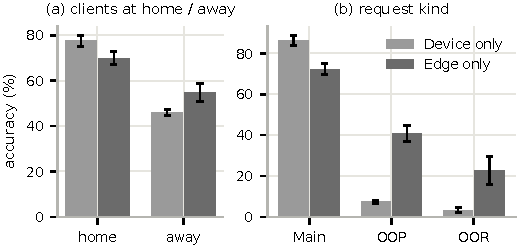
\includegraphics[width=\columnwidth]{motivation_exits}
\caption{Accuracy of the device exit alone (Device only) and the edge exit alone (Edge only) in the commute scenario S1 over the whole day. (a) Devices in their home cell and devices in another cell. (b) Requests from the device's own classes (Main), from classes learned only by other devices of the current cell (OOP), and from other classes (OOR). Error bars show the standard deviation over five seeds.}
\label{fig:motivation}
\end{figure}

Does one exit serve a moving device well throughout the day? Fig.~\ref{fig:motivation} answers this question by measuring each exit alone. Panel (a) splits devices by location, and panel (b) splits requests by their relation to the device. The device exit is more accurate at home (77.5\% against 69.9\%), and the edge exit is more accurate away from home (54.8\% against 45.9\%). Panel (b) shows the reason. The device exit is correct on 86.3\% of Main requests but on only 7.5\% of OOP requests and 3.3\% of OOR requests. The edge exit is correct on 72.3\%, 40.8\%, and 22.5\% of them. Each exit is better on one kind of request, and a moving device receives both kinds in the same day. A system that uses one exit for all requests therefore loses accuracy either at home or away.

\subsection{Choosing One Exit per Request}
\label{sec:choose}

The common way to use both exits is to choose one of them for each request. Split inference systems answer on the device when the device exit is confident and send the request to the edge otherwise~\cite{han2023splitgp,laskaridis2020spinn,teerapittayanon2016branchynet}. For this rule to work, the device exit must be uncertain on the requests that it cannot classify. We measure how well the entropy of the device exit separates OOP and OOR requests from Main requests. The area under the ROC curve (AUROC) is 0.64, where 0.5 means no separation. A personalized classifier places most of its probability on its user's classes even for a request from another class, a form of the overconfidence that neural classifiers show on inputs outside their training data~\cite{hendrycks2017baseline,guo2017calibration}.

The weak separation shows up in accuracy. With an entropy threshold of 0.8 nats, confidence-based offloading sends 92\% of requests to the edge and reaches 62.9\%. This is the same accuracy as always using the edge exit (62.9\%) and 1.3 points below always using the device exit (64.2\%). Choosing the exit with the lower entropy for each request performs similarly at 64.3\%. A per-request choice needs a per-request signal that tells the two kinds of requests apart, and the confidence of the device exit does not provide it.

\subsection{Adapting Personalization during Training}
\label{sec:training_side}

\begin{figure}[t]
\centering
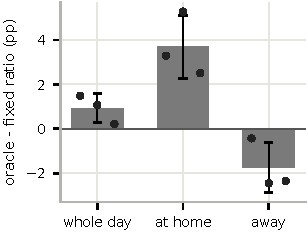
\includegraphics[width=0.62\columnwidth]{device_oracle}
\caption{Accuracy gain of an oracle that sets each device's personalization ratio from its true location (0.70 at home, 0.15 away) over a fixed ratio of 0.4 in S1, for all devices, devices at home, and devices away. Bars show the mean, error bars the standard deviation, and dots the three seeds.}
\label{fig:oracle}
\end{figure}

The other common remedy changes the model instead of the inference. A device could keep more of its local model when its traffic matches its own data and more of the shared model when it does not~\cite{deng2020apfl}. To measure how much this can give, we use an oracle that knows whether each device is at home. The oracle sets a personalization ratio of 0.70 at home and 0.15 away, while the baseline keeps 0.4 for every device.

Fig.~\ref{fig:oracle} shows the result. The oracle raises the accuracy of devices at home by 3.7 points, but it lowers the accuracy of devices away by 1.7 points, and the whole-day gain is 0.9 points. We attribute the loss away to the gain at home. Devices that keep more of their local model also send more specialized blocks into the cell average. The shared model of a cell then fits its residents more closely, and visitors who depend on that shared model lose accuracy. The benefit of personalization stays with one device, while its cost is spread over every device that shares the cell. A method without the oracle does even less. Learning the ratio of each device from its own training loss, as APFL does~\cite{deng2020apfl}, gives 62.9\% with the better of two learning rates, the same as the fixed ratio.

\subsection{Implications}
\label{sec:implications}

The measurements point to three requirements. First, a device needs both exits within the same day, because each exit is better on one kind of request. Second, the decision cannot rest on the confidence of the device exit for a single request. Third, the remedy should change only the answers of the device that needs it. If it changes the shared model instead, other devices pay for the gain. These requirements lead us to keep training unchanged and to combine the two exits at inference time, as Section~\ref{sec:design} describes.

\section{Related Work}
\label{sec:related}

\subsection{Split Inference and Early Exits}

Split computing places the first layers of a model on the device and the remaining layers on an edge server or the cloud, and chooses the split point from compute and network conditions~\cite{kang2017neurosurgeon,mao2017mecsurvey}. Early-exit networks attach classifiers to intermediate layers and stop when an exit is confident~\cite{teerapittayanon2016branchynet,kaya2019shallowdeep}. SPINN combines both ideas and decides at run time whether a request leaves at an on-device exit or continues to the cloud~\cite{laskaridis2020spinn}. In personalized split learning, SplitGP trains a personalized device-side model and a shared server-side model and sends a request to the server when the device-side output is uncertain~\cite{han2023splitgp}. These systems answer each request with one exit and use the confidence of an earlier exit to make that choice. Section~\ref{sec:choose} shows why this choice fails under mobility. The personalized exit is confident on classes it has never learned. DriftGate instead answers with both exits and uses confidence only to decide which requests are worth the cost of offloading.

Zero Time Waste (ZTW) reuses the predictions of earlier exits by combining them with later ones through a weighted geometric mean~\cite{wolczyk2021ztw}. All exits in ZTW are trained on the same data distribution, so none of them is systematically unaware of a class. The exits of personalized split learning differ in exactly this way. A geometric mean, which multiplies probabilities, lets the device exit's near-zero probability on an unlearned class cancel a correct edge answer. DriftGate uses an arithmetic average, which keeps the edge answer in that case, and it corrects the class bias of the edge exit before combining.

\subsection{Personalized Federated and Split Learning}

Personalized federated learning balances what a client learns from its own data with what it learns from others. APFL learns a mixture of a local and a global model, Ditto and pFedMe regularize local models toward a shared one, and FedRep shares a representation while keeping a local head~\cite{deng2020apfl,li2021ditto,tdinh2020pfedme,collins2021fedrep}. These methods set the balance during training. Section~\ref{sec:training_side} shows that, when users move independently, a training-time balance that helps residents of a cell lowers the accuracy of its visitors. Multi-cell split learning considers devices that move between overlapping cells and studies how the class mix of a cell affects training~\cite{rizwan2026splitomc}. Kim \emph{et al.} combine early exits with pretraining and online learning to handle label shift in personalized split federated learning~\cite{kim2025onlinepsfl}. DriftGate leaves training unchanged and acts only on how each request is answered.

Two methods combine a shared and a personalized classifier at inference time. FedRoD trains a generic head with a class-balanced loss and a personalized head on top of a shared feature extractor, and it predicts with the sum of the two heads' logits~\cite{chen2022fedrod}. Adding logits is equivalent to multiplying class probabilities, so the combination has the cancellation problem described above when one head has never learned a class. FedTHE ensembles a global and a personalized head with a weight chosen for each test sample by unsupervised objectives, including the entropy of the combined prediction~\cite{jiang2023fedthe}. Under mobility, a per-sample confidence objective favors the personalized exit on exactly the requests it gets wrong. DriftGate sets one weight per device from the average confidence of the two exits over recent requests, and it removes the class bias of the shared exit without changing its training. Our evaluation includes the combination rule of FedRoD and the entropy objective of FedTHE as baselines.

\subsection{Label Shift and Prior Correction}

When the class proportions of the test data differ from those of the training data, the outputs of a classifier can be corrected with Bayes' rule. Saerens \emph{et al.} estimate the new class proportions with expectation maximization (EM) and rescale the class probabilities~\cite{saerens2002adjusting}. Later work estimates the proportions from a confusion matrix~\cite{lipton2018bbse} or improves the calibration that the estimate depends on~\cite{alexandari2020mlls}. Logit adjustment applies the same correction with known class priors to train classifiers for long-tailed data~\cite{menon2021logit}. These methods correct one classifier toward an estimate of the current class mix. For a moving device, this mix changes with the device's location, and an estimate computed from the edge exit inherits the edge exit's bias against the device's own classes. DriftGate does not estimate the mix. It corrects the edge exit toward an even split between the device's own classes and all other classes, and lets the personalized device exit supply the device-specific preference. Our evaluation includes EM-based correction as a baseline.

\begin{table*}[t]
\centering
\caption{How inference methods use a personalized and a shared classifier. ``Correction'' refers to adjusting the shared classifier for the class mix of its training data.}
\label{tab:related}
\begin{adjustbox}{max width=\textwidth}
\begin{tabular}{l>{\raggedright\arraybackslash}p{3.0cm}>{\raggedright\arraybackslash}p{3.6cm}>{\raggedright\arraybackslash}p{4.0cm}>{\raggedright\arraybackslash}p{3.4cm}}
\toprule
Method & Classifiers used per request & How the answer is formed & Signal used at inference & Correction of the shared classifier \\
\midrule
SplitGP~\cite{han2023splitgp}, SPINN~\cite{laskaridis2020spinn} & One exit & Choose the device or the server exit & Entropy or confidence of the device exit for the request & None \\
ZTW~\cite{wolczyk2021ztw} & All exits up to the stopping point & Weighted geometric mean & Confidence of the combined prediction & None \\
FedRoD~\cite{chen2022fedrod} & Generic and personalized head & Sum of logits & None & Class-balanced training \\
FedTHE~\cite{jiang2023fedthe} & Global and personalized head & Weighted average, weight per sample & Unsupervised objectives on the test sample & None \\
EM correction~\cite{saerens2002adjusting} & One classifier & Rescaled class probabilities & Class mix estimated from recent predictions & Toward the estimated mix \\
DriftGate & Device and edge exit & Weighted average, weight per device & Average entropy of both exits over recent requests & Toward an even split of own and other classes, at inference \\
\bottomrule
\end{tabular}
\end{adjustbox}
\end{table*}

\section{System Model and Problem}
\label{sec:system}

\subsection{Devices, Cells, and Requests}

We consider $K$ mobile devices and $L$ cells. Each cell has an edge server that serves the devices inside its range, and neighboring cells can overlap. At time $t$, device $k$ belongs to a set $Z_k^t$ of one or two cells, and $Z_k^t$ changes as the device moves. Each device has a home cell where its user spends the night.

The data of device $k$ covers a set $M_k$ of its own classes out of $C$ classes. The user issues inference requests over the day. A request $x$ with class $y$ is a Main request if $y\in M_k$, an OOP request if $y$ belongs to the own classes of another device in the current cells, and an OOR request otherwise. The share of Main requests is high in the home cell and drops when the device visits other cells. The system never observes $y$, the kind of a request, or this share at inference time. The edge server knows $M_k$, because in split learning the labels of the training samples are sent to the edge.

\begin{table}[t]
\centering
\caption{Notation.}
\label{tab:notation}
\begin{adjustbox}{max width=\columnwidth}
\begin{tabular}{cl}
\toprule
Symbol & Meaning \\
\midrule
$k, z, c$ & Device, cell, and class index \\
$Z_k^t$ & Cells that device $k$ belongs to at time $t$ \\
$M_k$ & Own classes of device $k$ \\
$\pd(\cdot\,|\,x)$, $\pe(\cdot\,|\,x)$ & Class probabilities of the device and edge exits \\
$\pi_k$ & Class mix of the data that trained the edge exit for device $k$ \\
$a_k$ & Share of $M_k$ in $\pi_k$ \\
$\pec(\cdot\,|\,x)$ & Edge probabilities after prior correction \\
$r$ & Target share of classes outside $M_k$ in the correction \\
$w_k$ & Weight of the device exit when combining \\
$\Hd_k$, $\He_k$ & Mean entropy of the two exits on recent requests \\
$\tau$, $\beta$ & Offloading threshold and offloading budget \\
$\lambda$, $\Lambda$ & Device-to-cell and cell-to-global mixing ratios in training \\
\bottomrule
\end{tabular}
\end{adjustbox}
\end{table}

\subsection{Split Model and Training}
\label{sec:training}

The model of device $k$ consists of a device block $h_k$ and a device exit $f_k^{\mathrm{d}}$. The edge server of cell $z$ holds an edge block and an edge exit, written together as $f_z^{\mathrm{e}}$. For a request $x$, the device computes the feature $h_k(x)$ and the probabilities $\pd(\cdot\,|\,x)=\mathrm{softmax}(f_k^{\mathrm{d}}(h_k(x)))$. If the feature is sent to the edge, the edge returns $\pe(\cdot\,|\,x)=\mathrm{softmax}(f_z^{\mathrm{e}}(h_k(x)))$. A device that belongs to two cells receives the average of the two cells' logits.

Training follows multi-cell personalized split learning~\cite{han2023splitgp,rizwan2026splitomc}. We summarize the procedure used in our implementation. Training proceeds in rounds. In each round, device $k$ trains on labeled samples from its own classes with the loss
\begin{equation}
\mathcal{L}_k=\gamma\,\mathrm{CE}\!\left(f_k^{\mathrm{d}}(h_k(x)),y\right)+\frac{1-\gamma}{|Z_k^t|}\sum_{z\in Z_k^t}\mathrm{CE}\!\left(f_z^{\mathrm{e}}(h_k(x)),y\right),
\label{eq:loss}
\end{equation}
with $\gamma=0.5$. After local training, each cell averages the device blocks of its members. This average $\bar\theta_z$ and the edge block of the cell are each mixed with their averages over all cells, for example $\bar\theta_z\leftarrow\Lambda\bar\theta_z+(1-\Lambda)\bar\theta_{\mathrm{all}}$. Each device then installs
\begin{equation}
\theta_k\leftarrow\lambda\,\theta_k^{\mathrm{local}}+(1-\lambda)\,\bar\theta_{Z_k},
\label{eq:lambda}
\end{equation}
where $\theta_k^{\mathrm{local}}$ is its locally trained device block and $\bar\theta_{Z_k}$ is the average of its cells' blocks. A larger $\lambda$ keeps more of the local model. We use $\lambda=0.4$ and $\Lambda=0.5$ throughout. DriftGate does not change this procedure.

Because the edge block of a cell is trained on the samples of all its members, the edge exit learns the class mix of the cell. Let $n_z(c)$ be the number of samples of class $c$ used to train cell $z$ in the current round. We write the class mix that shaped the edge exit used by device $k$ as
\begin{equation}
\pi_k(c)=\frac{1}{|Z_k^t|}\sum_{z\in Z_k^t}\left[\Lambda\,\frac{n_z(c)}{\sum_{c'}n_z(c')}+(1-\Lambda)\,\frac{\sum_{z'}n_{z'}(c)}{\sum_{z',c'}n_{z'}(c')}\right],
\label{eq:pi}
\end{equation}
which follows the cell-to-global mixing of the edge blocks. The share of the device's own classes in this mix is $a_k=\sum_{c\in M_k}\pi_k(c)$. In the commute scenario, $a_k$ is about 0.25 on average.

\subsection{Inference Problem}

For each request $x$ of device $k$, an inference rule makes two decisions. It decides whether to offload, $o(x)\in\{0,1\}$, that is, whether to send $h_k(x)$ to the edge. It then produces an answer $\hat y(x)$ from $\pd(\cdot\,|\,x)$ and, if $o(x)=1$, from $\pe(\cdot\,|\,x)$. The rule may use information that the device and the edge already hold, such as recent outputs, $M_k$, and $\pi_k$, but not labels at inference time and not the location of the device.

Let $\mathcal{T}$ be the evaluation times of a day and $\mathcal{K}_t$ the devices that issue requests at time $t$. The accuracy of a rule over the day is
\begin{equation}
A=\frac{1}{|\mathcal{T}|}\sum_{t\in\mathcal{T}}\frac{1}{|\mathcal{K}_t|}\sum_{k\in\mathcal{K}_t}\Pr\!\left[\hat y(x)=y\,\middle|\,k,t\right].
\label{eq:accuracy}
\end{equation}
The goal is to maximize $A$ while the share of offloaded requests stays within a budget $\beta$, so that $\mathbb{E}[o(x)]\le\beta$. When $\beta=1$, every request can use both exits, and the problem reduces to combining the two probability vectors well.

\section{DriftGate}
\label{sec:design}

\begin{figure*}[t]
\centering
\resizebox{0.98\textwidth}{!}{%
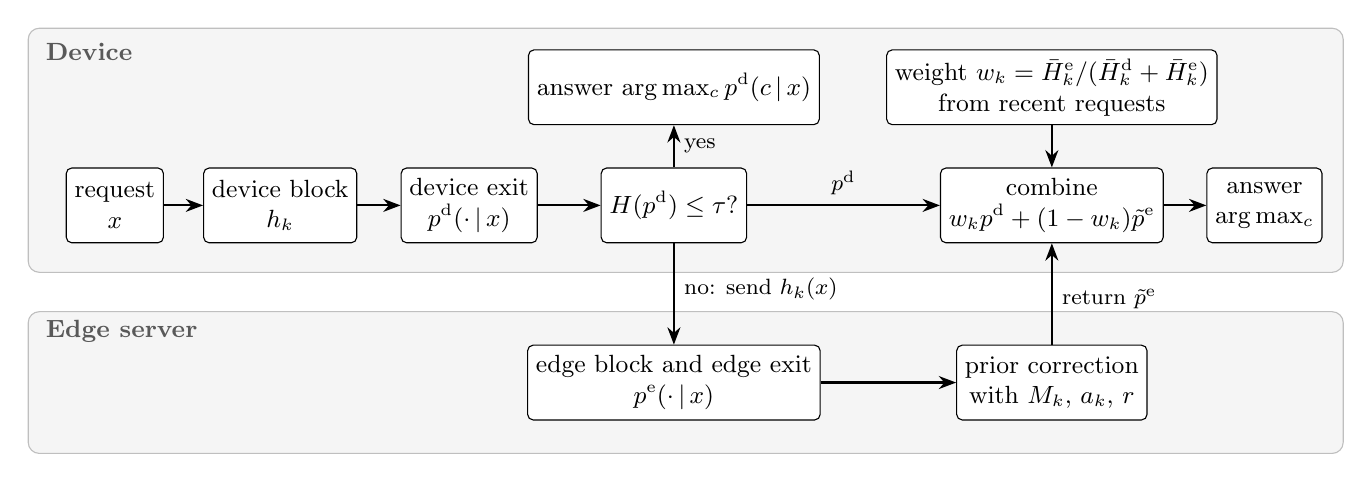
\begin{tikzpicture}[font=\small,
  box/.style={draw, rounded corners=2pt, align=center, minimum height=0.95cm, inner sep=3pt, fill=white},
  arr/.style={-{Stealth[length=2.2mm]}, thick},
  lane/.style={draw=gray!50, fill=gray!8, rounded corners=4pt}]
  \fill[gray!8, draw=gray!50, rounded corners=4pt] (-1.1,-0.85) rectangle (15.6,2.25);
  \fill[gray!8, draw=gray!50, rounded corners=4pt] (-1.1,-3.15) rectangle (15.6,-1.35);
  \node[anchor=west, text=gray!70!black, font=\small\bfseries] at (-1.0,1.95) {Device};
  \node[anchor=west, text=gray!70!black, font=\small\bfseries] at (-1.0,-1.6) {Edge server};
  \node[box] (in) at (0,0) {request\\$x$};
  \node[box] (db) at (2.1,0) {device block\\$h_k$};
  \node[box] (de) at (4.5,0) {device exit\\$\pd(\cdot\,|\,x)$};
  \node[box] (chk) at (7.1,0) {$H(\pd)\le\tau$?};
  \node[box] (loc) at (7.1,1.5) {answer $\arg\max_c \pd(c\,|\,x)$};
  \node[box] (win) at (11.9,1.5) {weight $w_k=\He_k/(\Hd_k+\He_k)$\\from recent requests};
  \node[box] (comb) at (11.9,0) {combine\\$w_k\pd+(1-w_k)\pec$};
  \node[box] (ans) at (14.6,0) {answer\\$\arg\max_c$};
  \node[box] (eb) at (7.1,-2.25) {edge block and edge exit\\$\pe(\cdot\,|\,x)$};
  \node[box] (pc) at (11.9,-2.25) {prior correction\\with $M_k$, $a_k$, $r$};
  \draw[arr] (in) -- (db);
  \draw[arr] (db) -- (de);
  \draw[arr] (de) -- (chk);
  \draw[arr] (chk) -- node[right, font=\footnotesize] {yes} (loc);
  \draw[arr] (chk.south) -- node[pos=0.45, right, font=\footnotesize] {no: send $h_k(x)$} (eb.north);
  \draw[arr] (chk.east) -- node[above, font=\footnotesize] {$\pd$} (comb.west);
  \draw[arr] (eb) -- (pc);
  \draw[arr] (pc.north) -- node[pos=0.45, right, font=\footnotesize] {return $\pec$} (comb.south);
  \draw[arr] (win) -- (comb);
  \draw[arr] (comb) -- (ans);
\end{tikzpicture}}
\caption{Inference with DriftGate. The device answers a request locally when its exit is confident. Otherwise it sends the intermediate feature to the edge, which returns class probabilities corrected for the class mix of the cell, and the device answers with a weighted average of both exits. The weight comes from the mean entropy of the two exits on the device's recent requests.}
\label{fig:overview}
\end{figure*}

DriftGate changes only how a request is answered. It keeps the trained device and edge models as they are and adds three steps that follow from Section~\ref{sec:motivation}. It combines the two exits instead of choosing one, it corrects the edge exit for the class mix of its cell, and it sets the weight of each exit without labels. A fourth step limits offloading to the requests where the edge is most useful. Fig.~\ref{fig:overview} shows the resulting path of a request.

\subsection{Combining the Two Exits}
\label{sec:combine}

Section~\ref{sec:complementary} showed that the device exit is accurate on Main requests and the edge exit on OOP and OOR requests, and Section~\ref{sec:choose} showed that the device exit cannot tell these requests apart by its own confidence. DriftGate therefore uses both exits on every offloaded request and answers with
\begin{equation}
\hat y(x)=\arg\max_c\; w_k\,\pd(c\,|\,x)+(1-w_k)\,\pec(c\,|\,x),
\label{eq:combine}
\end{equation}
where $\pec$ is the corrected edge output of Section~\ref{sec:correct} and $w_k\in[0,1]$ is the weight of the device exit.

The choice of an arithmetic average matters. On a Main request, the device exit puts a large probability on the correct class, and the average follows it unless the edge exit is confident in another class. On an OOP request, the device exit has never learned the correct class and spreads its probability over its own classes, while the edge exit puts a large probability on the correct class. The average keeps $(1-w_k)$ times this probability, so the edge answer still wins when the edge exit is confident. A product of probabilities, which is what adding logits computes~\cite{chen2022fedrod,wolczyk2021ztw}, behaves differently. Because the device exit assigns the correct class a probability close to zero, the product removes the edge exit's answer however confident the edge exit is. The literature on combining probability forecasts describes the same contrast between linear and logarithmic pooling~\cite{genest1986combining}. Section~\ref{sec:ablation} confirms that the average is more accurate than the product in our settings.

\subsection{Correcting the Edge Exit for Its Cell}
\label{sec:correct}

The average in Eq.~\eqref{eq:combine} works only if the edge exit gives the device's own classes a fair chance. It does not do so by default. A classifier trained on data with class mix $\pi$ produces probabilities proportional to $p(x\,|\,c)\,\pi(c)$. The edge exit is trained on the class mix $\pi_k$ of the cell (Eq.~\eqref{eq:pi}), in which the device's own classes have a share $a_k$ of about 0.25 in the commute scenario. A device at home, however, receives own-class requests about 88\% of the time. The edge exit therefore discounts exactly the classes that dominate the device's traffic, and on a Main request it often prefers a class of another device in the cell.

DriftGate removes this discount with Bayes' rule~\cite{saerens2002adjusting}. It replaces the training mix $\pi_k$ with a target mix that keeps the relative frequencies within the device's own classes and within the other classes, but gives the other classes a total share $r$:
\begin{equation}
\pec(c\,|\,x)\propto
\begin{cases}
\pe(c\,|\,x)\,\dfrac{1-r}{a_k}, & c\in M_k,\\[2mm]
\pe(c\,|\,x)\,\dfrac{r}{1-a_k}, & c\notin M_k,
\end{cases}
\label{eq:correct}
\end{equation}
normalized to sum to one. We set $r=1/2$, so the corrected edge exit treats the device's own classes and all other classes as equally likely before seeing the request.

We use this even split instead of an estimate of the device's current mix for three reasons. First, the true share changes with the device's location, from about 0.115 at home to about 0.51 away in the commute scenario, and the edge cannot observe it. Second, an estimate computed from the edge exit inherits the bias that the correction is meant to remove. In our development runs, the EM estimate of Saerens \emph{et al.}~\cite{saerens2002adjusting} gave 0.23 for devices away from home, where the true share was 0.51. Third, the combined answer does not need the edge exit to know the device's preference for its own classes, because the device exit already carries that preference. The edge exit only needs to stop discounting those classes. The correction uses only $M_k$ and $\pi_k$, which the edge already holds from training.

\subsection{Setting the Weight without Labels}
\label{sec:weight}

The weight $w_k$ decides how much the device exit counts in Eq.~\eqref{eq:combine}. Its best value depends on the model and the split point. With a small device block, the edge exit is the stronger classifier on most requests. With a large device block, such as the first half of a ResNet-18, the device exit can be stronger than the edge exit overall. A single fixed weight cannot suit both cases, and labels are not available to tune it after deployment.

DriftGate sets the weight from how confident the two exits are on the device's recent traffic. Let $\Hd_k$ and $\He_k$ be the mean entropies of the device exit and the edge exit over a window of recent offloaded requests of device $k$. DriftGate uses
\begin{equation}
w_k=\frac{\He_k}{\Hd_k+\He_k},
\label{eq:weight}
\end{equation}
so the exit that has been more confident on this device's requests receives the larger weight. Section~\ref{sec:choose} showed that the confidence of the device exit on one request is not reliable. The mean over many requests answers a different question. It does not try to identify the kind of each request, but measures which exit is generally sharper for this device, model, and split point. Until the window holds eight requests, DriftGate uses $w_k=1/2$. In the commute scenario, $w_k$ is about 0.42 on average.

\subsection{Offloading Only Uncertain Requests}
\label{sec:offload}

Combining requires the edge output, so every request that DriftGate combines must be offloaded. When the network or the edge is a bottleneck, the device can answer some requests alone. DriftGate keeps the confidence of the device exit for this purpose. A request with $H(\pd(\cdot\,|\,x))\le\tau$ is answered with the device exit, and the other requests are offloaded and combined. The threshold $\tau$ follows the offloading budget $\beta$, for example as the $(1-\beta)$ quantile of recent device-exit entropies. The confidence of the device exit is too weak to choose the exit that answers a request, but it is useful for ranking which requests gain least from the edge. Requests with very low device-exit entropy are more often Main requests that the device exit already answers correctly, so they gain least from the edge. Since only offloaded requests have an edge output, $\He_k$ is computed over offloaded requests only.

\begin{algorithm}[t]
\caption{DriftGate inference for a request $x$ of device $k$}
\label{alg:driftgate}
\begin{algorithmic}[1]
\REQUIRE threshold $\tau$, window of recent entropies of device $k$; edge holds $M_k$, $\pi_k$, and $r$
\STATE compute $h_k(x)$ and $\pd(\cdot\,|\,x)$ on the device
\IF{$H(\pd(\cdot\,|\,x))\le\tau$}
  \RETURN $\arg\max_c \pd(c\,|\,x)$
\ENDIF
\STATE send $h_k(x)$ to the edge server
\STATE \textit{edge:} compute $\pe(\cdot\,|\,x)$, $H(\pe(\cdot\,|\,x))$, and $\pec(\cdot\,|\,x)$ by Eq.~\eqref{eq:correct}; return $\pec$ and the entropy
\STATE add $H(\pd)$ and $H(\pe)$ to the window and update $\Hd_k$, $\He_k$
\STATE $w_k\leftarrow \He_k/(\Hd_k+\He_k)$, or $1/2$ if the window holds fewer than eight requests
\RETURN $\arg\max_c\; w_k\pd(c\,|\,x)+(1-w_k)\pec(c\,|\,x)$
\end{algorithmic}
\end{algorithm}

\subsection{Deployment and Cost}
\label{sec:cost}

Algorithm~\ref{alg:driftgate} summarizes DriftGate. The edge applies the correction because it already holds $M_k$ and the class counts of its training data. Instead of a single label, it returns $C$ corrected probabilities and one entropy value, which is 44 bytes for ten classes in single precision. The device keeps two running means for the weight and computes one weighted average of two $C$-dimensional vectors per offloaded request. On a server CPU, the correction and the combination take 3.2\,$\mu$s for one request. Training, the models, and the uplink payload stay unchanged.

\section{Evaluation}
\label{sec:evaluation}

We ask five questions. Is DriftGate more accurate than existing inference rules under mobility (Section~\ref{sec:overall})? Which devices, requests, and times of day does the gain come from (Section~\ref{sec:where})? How much accuracy does it keep when fewer requests are offloaded (Section~\ref{sec:eval_offload})? Which parts of the design produce the gain (Section~\ref{sec:ablation})? And how does it behave at larger scale, for the least accurate devices, and on real devices (Sections~\ref{sec:scale} and~\ref{sec:device})?

\subsection{Setup}
\label{sec:setup}

\textbf{Settings.} Table~\ref{tab:settings} lists the settings. The commute scenario S1 places five cells with a 1\,km edge range, four residential cells and one hub, and 50 devices whose users walk from home to the hub and back over a day from 05:00 to 20:00. Training runs in 150 rounds of six minutes. Every device is at home at 05:00, and during the day about 35\% are, while the hub holds up to 32 devices. About 14\% of the devices are inside two cells at a time. S2 replaces the synthetic paths with 50 weekday user-days from the GeoLife trajectories~\cite{zheng2010geolife} and places five edges by $k$-means over the traces. S2 has a weaker commute pattern, and about 60\% of its devices stay at home during the day. S1-fast moves the S1 users at vehicle speed, and partial participation lets a random half of the devices train in each round. Two further settings change the class mix of all devices together. In the stepwise change, cell membership is fixed while the share parameter $\rho$ defined below rises from 0 to 0.8 and returns to 0 in five phases. In random mobility, devices move between cells by a Gauss--Markov model~\cite{liang1999gaussmarkov}, and $\rho$ changes from 0 to 0.8 halfway through the run. CIFAR-100 repeats S1 with 100 classes, and ResNet-18 repeats the stepwise change with a ResNet-18~\cite{he2016resnet} split in the middle. Section~\ref{sec:scale} repeats the S1 layout to reach 200 and 500 devices.

\begin{table}[t]
\centering
\caption{Evaluation settings. All settings except the scale study use 50 devices and five cells.}
\label{tab:settings}
\begin{adjustbox}{max width=\columnwidth}
\begin{tabular}{l>{\raggedright\arraybackslash}p{4.3cm}lc}
\toprule
Setting & Movement and class mix & Data, model & Seeds \\
\midrule
S1 (commute) & Walking commute between four residential cells and a hub & CIFAR-10, CNN & 5 \\
S2 (GeoLife) & 50 user-days of GeoLife traces & CIFAR-10, CNN & 3 \\
S1-fast & S1 at vehicle speed & CIFAR-10, CNN & 3 \\
Partial participation & S1, half of the devices train per round & CIFAR-10, CNN & 3 \\
Stepwise change & Fixed cells, $\rho$: 0, 0.4, 0.8, 0.4, 0 for all devices & CIFAR-10, CNN & 5 \\
Random mobility & Gauss--Markov movement, $\rho$: 0 then 0.8 & CIFAR-10, CNN & 3 \\
CIFAR-100 & S1 with 100 classes & CIFAR-100, CNN & 3 \\
ResNet-18 & Stepwise change & CIFAR-10, ResNet-18 & 3 \\
Scale & S1 layout repeated, 200 and 500 devices & CIFAR-10, CNN & 3 \\
\bottomrule
\end{tabular}
\end{adjustbox}
\end{table}

\textbf{Data and requests.} Each device holds two own classes of CIFAR-10~\cite{krizhevsky2009cifar}, or 20 of CIFAR-100. In S1, a device holds 620 to 2,857 training images. The requests of a device in an evaluation round are test images. For every Main request, a device receives on average $\rho$ OOP requests and $0.3\rho$ OOR requests. In the mobility settings, $\rho=0.1$ in the device's home cell and $\rho=0.8$ elsewhere, so OOP and OOR requests make up about 11.5\% and 51\% of the traffic.

\textbf{Models and training.} The CNN has a device block of 0.13\,M parameters, a device exit of 0.15\,M parameters, and an edge block and exit of 1.38\,M parameters. Its intermediate feature has $128\times8\times8$ values (32\,KB in single precision). All models are trained from random initialization with SGD (learning rate 0.01, weight decay $10^{-4}$, batch size 32, three local epochs per round) and the procedure of Section~\ref{sec:training} with $\lambda=0.4$ and $\Lambda=0.5$. Because training starts at the beginning of the day, the first evaluation rounds also cover the early phase of training.

\textbf{Inference rules.} All rules answer the same requests with the same trained models.
\begin{itemize}
\item \emph{SplitGP} answers with the device exit if its entropy is at most 0.8 nats and otherwise with the edge exit, as in confidence-based offloading~\cite{han2023splitgp}.
\item \emph{Device only} and \emph{Edge only} always use one exit.
\item \emph{Average} answers with the mean of the two probability vectors.
\item \emph{FedRoD} adds the logits of the two exits, which is the combination rule of FedRoD~\cite{chen2022fedrod}.
\item \emph{FedTHE} uses, for each request, the exit with the lower entropy. This is the solution of FedTHE's entropy objective over the ensemble weight~\cite{jiang2023fedthe}, because the entropy of a mixture is concave in the weight and is minimized at one end. FedTHE's feature-alignment term does not apply, because the two exits use different features.
\item \emph{ZTW} answers with the device exit when its largest probability exceeds a threshold and otherwise with the geometric mean of both exits~\cite{wolczyk2021ztw}. The threshold gives the same offloading ratio as SplitGP.
\item \emph{Label-shift EM} corrects the edge exit with the share of other classes estimated by EM on the device's recent requests and answers with the corrected edge exit~\cite{saerens2002adjusting}.
\item \emph{Learned weight} combines the exits with a per-request weight from a logistic regression on nine label-free features, such as the confidence of each exit and their agreement. The regression is trained with labels from separate development runs, which gives per-request weighting an advantage that a deployed system would not have.
\end{itemize}
DriftGate uses $r=1/2$ and a window of at least eight requests. In the simulation, the window holds the earlier requests of the current evaluation round, or the requests of the previous one when fewer than eight have arrived. Except in Section~\ref{sec:eval_offload}, DriftGate, Average, FedRoD, Label-shift EM, and Learned weight offload every request, and ZTW offloads the same share as SplitGP. The value of $r$, the window size, and the logistic regression were fixed on development runs whose seeds are not used in this section.

\textbf{Metric.} We report the accuracy of Eq.~\eqref{eq:accuracy} over the whole run. Evaluation takes place every five rounds in the mobility settings and every ten rounds in the stepwise change and random mobility. We report the mean over seeds, and differences are computed per seed before averaging.

\subsection{Overall Accuracy}
\label{sec:overall}

\begin{table*}[t]
\centering
\caption{Accuracy (\%) over the whole run. The last three rows give the gain of DriftGate over confidence-based offloading (SplitGP), its gain over the most accurate other rule in each setting, and that rule. Gains are the mean and standard deviation of the per-seed difference.}
\label{tab:main}
\begin{adjustbox}{max width=\textwidth}
\begin{tabular}{lcccccccc}
\toprule
Rule & S1 & S2 & S1-fast & Partial part. & Stepwise & Random mob. & CIFAR-100 & ResNet-18 \\
\midrule
SplitGP & 62.87 & 65.18 & 63.33 & 56.45 & 65.17 & 58.56 & 35.84 & 59.21 \\
Device only & 64.16 & 69.04 & 64.39 & 61.75 & 68.93 & 67.71 & 33.93 & 66.39 \\
Edge only & 62.91 & 65.24 & 63.38 & 56.44 & 65.20 & 58.61 & 35.84 & 57.04 \\
Average & 67.32 & 69.88 & 68.06 & 62.64 & 71.44 & 69.58 & 38.15 & 66.39 \\
FedRoD & 67.37 & 70.07 & 68.12 & 62.94 & 71.39 & 69.23 & 39.83 & 66.00 \\
FedTHE & 64.35 & 66.65 & 64.90 & 58.10 & 68.42 & 64.22 & 35.89 & 66.54 \\
ZTW & 67.36 & 70.06 & 68.11 & 62.94 & 71.38 & 69.22 & 39.83 & 65.99 \\
Label-shift EM & 64.84 & 68.63 & 65.41 & 60.45 & 67.59 & 65.42 & 40.44 & 61.73 \\
Learned weight & 66.81 & 68.59 & 67.52 & 62.02 & 70.69 & 68.55 & 37.54 & 63.61 \\
DriftGate & \textbf{68.31} & \textbf{71.70} & \textbf{68.96} & \textbf{64.82} & \textbf{72.36} & \textbf{71.09} & \textbf{41.29} & \textbf{66.64} \\
\midrule
Gain over SplitGP & 5.45 (0.47) & 6.52 (2.77) & 5.63 (0.38) & 8.37 (0.15) & 7.18 (0.77) & 12.53 (1.08) & 5.45 (0.67) & 7.43 (2.17) \\
Gain over best other & 0.95 (0.57) & 1.63 (1.04) & 0.84 (0.25) & 1.88 (0.59) & 0.92 (0.26) & 1.52 (0.53) & 0.85 (0.31) & 0.10 (0.61) \\
Best other rule & FedRoD & FedRoD & FedRoD & FedRoD & Average & Average & Label-shift EM & FedTHE \\
\bottomrule
\end{tabular}
\end{adjustbox}
\end{table*}

Is DriftGate more accurate than the existing ways of answering requests? Table~\ref{tab:main} compares the ten rules in the eight settings. The rules fall into two groups. Rules that choose one exit per request, namely SplitGP and FedTHE, do not rise clearly above the better single exit and often fall below it. Rules that combine the exits, namely Average, FedRoD, and ZTW, are 2 to 11 points above SplitGP. DriftGate is the most accurate rule in all eight settings. Its gain over SplitGP ranges from 5.4 points in S1 and CIFAR-100 to 12.5 points in random mobility, and its gain over the most accurate other rule ranges from 0.1 to 1.9 points.

The strongest alternative changes from setting to setting. It is FedRoD in the four settings built on individual movement, Average when the class mix changes for all devices together, Label-shift EM in CIFAR-100, and FedTHE with ResNet-18. No existing rule is the best choice across settings, whereas DriftGate is the most accurate in every one, with the largest margins under partial participation (1.9 points) and in S2 (1.6 points). In CIFAR-100, where each device owns 20 of 100 classes, the strongest alternative is Label-shift EM, which also corrects the edge exit. This confirms that the class bias of the edge exit matters, and DriftGate is 0.9 points above it because it combines the corrected edge exit with the device exit. The smallest gain appears with ResNet-18, whose large device block makes the device exit more accurate than the edge exit (66.4\% against 57.0\%). With little to gain from the edge, every reasonable rule ends close to the device exit, and DriftGate remains the most accurate by 0.1 points.

The combining rules also show why per-request weighting is not the answer. The learned weight uses labels from development runs to predict, for each request, which exit to trust. It is still 1.5 points below DriftGate in S1 and 3.1 points below in S2, because label-free features do not identify the kind of a single request reliably. A weight that reflects the device's recent traffic is enough, provided that the edge exit is corrected first.

\subsection{Where the Gain Comes From}
\label{sec:where}

\begin{figure*}[t]
\centering
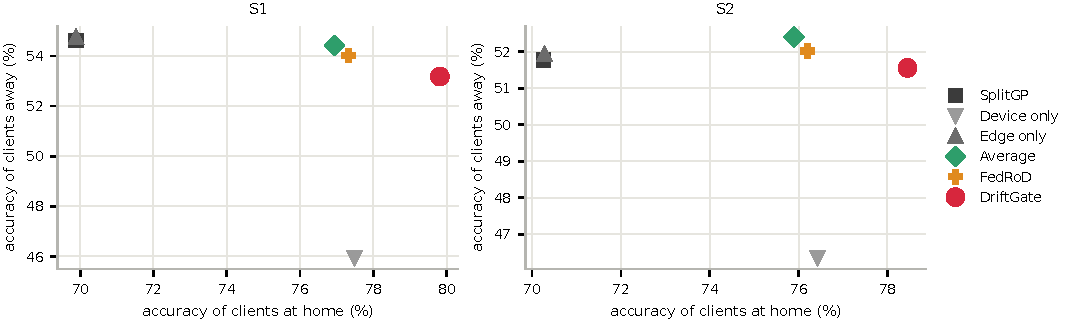
\includegraphics[width=0.92\textwidth]{home_away}
\caption{Accuracy of devices in their home cell against accuracy of devices in another cell for six inference rules in S1 (left) and S2 (right), over the whole day.}
\label{fig:home_away}
\end{figure*}

\begin{table}[t]
\centering
\caption{Accuracy (\%) by request kind in S1 and S2 over the whole day.}
\label{tab:kinds}
\begin{adjustbox}{max width=\columnwidth}
\begin{tabular}{llccc}
\toprule
Setting & Rule & Main & OOP & OOR \\
\midrule
\multirow{6}{*}{S1} & SplitGP & 72.31 & 40.41 & 22.37 \\
 & Device only & 86.31 & 7.49 & 3.30 \\
 & Edge only & 72.27 & 40.79 & 22.52 \\
 & Average & 82.36 & 29.34 & 15.45 \\
 & FedRoD & 83.01 & 27.72 & 14.76 \\
 & DriftGate & 86.94 & 21.63 & 10.68 \\
\midrule
\multirow{6}{*}{S2} & SplitGP & 73.46 & 46.39 & 8.72 \\
 & Device only & 84.65 & 15.29 & 1.69 \\
 & Edge only & 73.42 & 46.92 & 8.82 \\
 & Average & 80.83 & 38.50 & 6.18 \\
 & FedRoD & 81.32 & 37.11 & 5.85 \\
 & DriftGate & 84.70 & 30.63 & 4.86 \\
\bottomrule
\end{tabular}
\end{adjustbox}
\end{table}

Which devices benefit from DriftGate? Fig.~\ref{fig:home_away} places each rule by the accuracy of devices at home (horizontal axis) and away (vertical axis). The single exits sit at opposite corners. The device exit is accurate at home and poor away, and the edge exit and SplitGP are the reverse. DriftGate moves to the right of every other rule. In S1, devices at home reach 79.8\%, which is 2.3 points above the device exit alone and 2.5 points above FedRoD. Devices away reach 53.2\%, within 1.6 points of the edge exit alone. In S2 the pattern is the same. Devices at home are 2.0 points above the device exit alone, and devices away are 0.4 points below the edge exit alone. DriftGate thus keeps the strength of the device exit at home while giving up little of the edge exit's accuracy away.

Table~\ref{tab:kinds} shows the same result by request kind. On Main requests, DriftGate is as accurate as the device exit alone (86.9\% against 86.3\% in S1), whereas Average and FedRoD lose 3 to 4 points there. The prior correction is what closes this gap, because it stops the edge exit from pulling Main requests toward the classes of other devices. On OOP and OOR requests, DriftGate stays well above the device exit, though below the edge exit. Main requests make up most of a device's traffic over the day, so this trade raises overall accuracy.

\begin{figure*}[t]
\centering
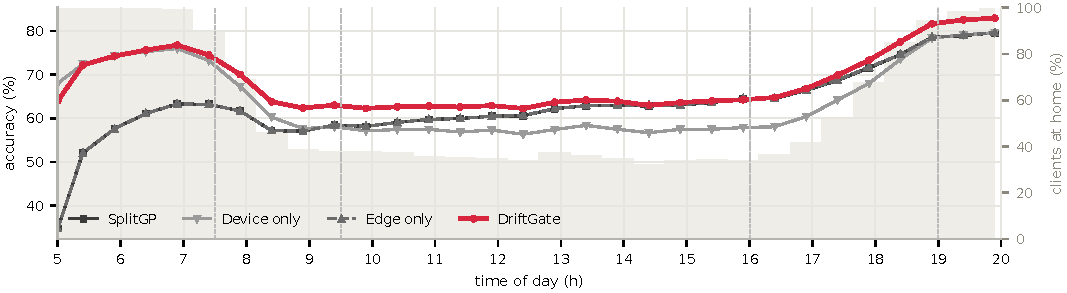
\includegraphics[width=0.92\textwidth]{time_of_day}
\caption{Accuracy over the day in S1 for SplitGP, the device exit alone, the edge exit alone, and DriftGate. The shaded background shows the share of devices in their home cell (right axis). Dashed lines separate the pre-commute, commute, daytime, return, and evening periods.}
\label{fig:time}
\end{figure*}

When during the day does the gain appear? Fig.~\ref{fig:time} follows the accuracy of four rules through the day in S1. Before the commute, almost every device is at home and DriftGate follows the device exit (72.9\% against 73.2\%). In these early hours the edge exit is still in its first rounds of training, and SplitGP, which sends most requests to it, stays at 55.3\%. During the day, when most devices are away, the device exit falls below the edge exit, and DriftGate stays above both exits from the commute until the evening. Its lead over the better single exit is 4.0 points during the commute, 1.7 points during the day, 1.5 points on the way back, and 3.4 points in the evening. The commute is when a device's traffic changes fastest, and it is also when combining the two exits helps most.

\subsection{Accuracy and Offloading}
\label{sec:eval_offload}

\begin{figure*}[t]
\centering
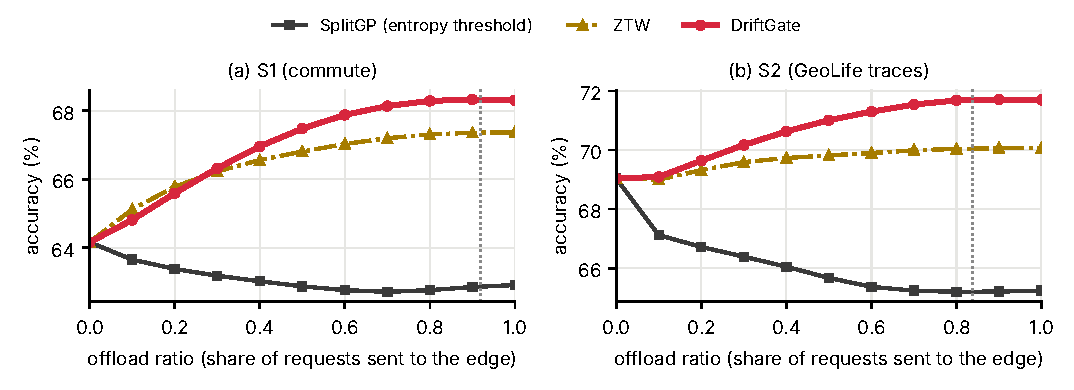
\includegraphics[width=0.92\textwidth]{offload_curves}
\caption{Accuracy against the offloading ratio when only requests on which the device exit is uncertain are sent to the edge. SplitGP and DriftGate offload requests whose device-exit entropy exceeds a threshold, and ZTW offloads requests whose largest device-exit probability is below a threshold. SplitGP answers the offloaded requests with the edge exit, ZTW with the geometric mean of both exits, and DriftGate with its combination. The dotted line marks the offloading ratio of SplitGP at its default threshold of 0.8 nats.}
\label{fig:offload}
\end{figure*}

How much accuracy does DriftGate keep when fewer requests can be offloaded? Fig.~\ref{fig:offload} varies the offloading threshold of each rule and plots accuracy against the share of requests sent to the edge. The threshold is on the device-exit entropy for SplitGP and DriftGate and on the largest device-exit probability for ZTW. All curves start from the device exit alone at an offloading ratio of zero. For SplitGP, sending more requests to the edge lowers accuracy in both scenarios, because the additional requests are more often Main requests, which the device exit answers better than the edge exit. ZTW and DriftGate improve as they offload more, since both use the device exit's output when they combine. DriftGate is above ZTW at every offloading ratio of 0.3 or more in all eight settings.

The curves also show how much offloading DriftGate needs. In S1, DriftGate exceeds every other rule in Table~\ref{tab:main}, most of which use the edge for every request, once it offloads 48\% of requests. In S2 it needs 28\%. Across the eight settings, this point lies between 11\% and 50\% in seven settings. CIFAR-100 needs 85\%, because with 100 classes the device exit is weak on its own and most requests benefit from the edge. SplitGP, by comparison, offloads 92\% of the requests in S1 and 84\% in S2 at its default threshold. In seven of the eight settings, DriftGate can therefore halve the traffic to the edge and still be more accurate than any rule that uses the edge for every request.

\subsection{Ablation}
\label{sec:ablation}

\begin{table}[t]
\centering
\caption{Accuracy (\%) of DriftGate and variants that remove one design choice.}
\label{tab:ablation}
\begin{adjustbox}{max width=\columnwidth}
\begin{tabular}{lccc}
\toprule
Variant & S1 & Random mob. & ResNet-18 \\
\midrule
DriftGate & \textbf{68.31} & \textbf{71.09} & 66.64 \\
Fixed weight $w=0.2$ & 68.16 & 70.51 & 64.02 \\
Fixed weight $w=0.5$ & 68.13 & 70.96 & \textbf{66.71} \\
No correction, $w=0.2$ & 64.75 & 63.78 & 61.25 \\
No correction, $w=0.5$ (Average) & 67.32 & 69.58 & 66.39 \\
Correction and product & 67.90 & 70.78 & 66.59 \\
\bottomrule
\end{tabular}
\end{adjustbox}
\end{table}

Which parts of DriftGate produce the gain? Table~\ref{tab:ablation} removes one choice at a time in S1, random mobility, and ResNet-18. Removing the prior correction costs the most. With $w=0.2$, accuracy drops by 3.4 points in S1 and by 6.7 points in random mobility. Without the correction, the edge exit pulls Main requests toward the classes of other devices, and giving the edge exit more weight makes this worse.

The weight matters differently for each model. A fixed weight of 0.2 is 2.6 points below DriftGate on ResNet-18, where the device exit is the stronger classifier. A fixed weight of 0.5 suits ResNet-18 but is 0.1 to 0.2 points below DriftGate on the CNN settings. The label-free weight of Eq.~\eqref{eq:weight} is at least as accurate as the better fixed weight in the two CNN settings and 0.07 points below it on ResNet-18, without being tuned for either model. Replacing the average with a product, which is how FedRoD and ZTW combine their outputs, lowers accuracy in all three settings even with the correction in place. This matches the argument of Section~\ref{sec:combine}. A product lets the device exit's near-zero probabilities on unlearned classes overrule the edge exit.

\subsection{Scale and the Least Accurate Devices}
\label{sec:scale}

\begin{table}[t]
\centering
\caption{Accuracy (\%) as the number of devices grows. The last column gives the offloading ratio at which DriftGate first matches the accuracy of SplitGP.}
\label{tab:scale}
\begin{adjustbox}{max width=\columnwidth}
\begin{tabular}{rcccccc}
\toprule
Devices & Cells & SplitGP & DriftGate & Gain & \multicolumn{2}{c}{Offloading ratio} \\
\cmidrule(lr){6-7}
 & & & & & SplitGP & DriftGate \\
\midrule
50 & 5 & 62.87 & 68.31 & 5.45 & 0.920 & 0.000 \\
200 & 20 & 65.26 & 69.00 & 3.73 & 0.949 & 0.218 \\
500 & 50 & 67.03 & 70.11 & 3.08 & 0.955 & 0.299 \\
\bottomrule
\end{tabular}
\end{adjustbox}
\end{table}

Does the gain hold in larger deployments? Table~\ref{tab:scale} repeats the S1 layout with 200 and 500 devices. DriftGate stays 3.1 to 5.4 points above SplitGP. With 200 and 500 devices, the device exit alone is less accurate than SplitGP, so DriftGate needs some offloading to match it. Even with 500 devices, DriftGate matches the accuracy of SplitGP while offloading 30\% of requests instead of 95.5\%. The edge work per request does not depend on the number of devices, because the correction uses only the class counts of the device's cells.

\begin{table}[t]
\centering
\caption{Accuracy (\%) of the 10\% least accurate devices, averaged over evaluation rounds.}
\label{tab:bottom}
\begin{adjustbox}{max width=\columnwidth}
\begin{tabular}{lcccc}
\toprule
Setting & SplitGP & Average & FedRoD & DriftGate \\
\midrule
S1 & 40.98 & 46.62 & 46.38 & \textbf{48.00} \\
S2 & 39.53 & 45.89 & 45.88 & \textbf{47.43} \\
S1-fast & 41.61 & 47.99 & 47.66 & \textbf{49.37} \\
Partial participation & 31.28 & 39.27 & 39.67 & \textbf{43.24} \\
\bottomrule
\end{tabular}
\end{adjustbox}
\end{table}

Does the average gain hide devices that do worse? Table~\ref{tab:bottom} reports the accuracy of the 10\% least accurate devices in each evaluation round. DriftGate raises this accuracy by 7.0 to 12.0 points over SplitGP and by 1.4 to 3.6 points over the strongest combining rule. The gain therefore reaches the devices that are served worst, not only the average device.

\subsection{Cost on Mobile Devices}
\label{sec:device}

\todo{Replace this subsection with the measured values. The structure and the expected values below follow the latency model of Section~\ref{sec:cost}; all red numbers are estimates.}

\textbf{Setup.} We measure the inference path on two smartphones, \todo{Samsung Galaxy model 1} and \todo{model 2}, and on an NVIDIA Jetson \todo{model} board. The device block and the device exit run with \todo{runtime, e.g., PyTorch Mobile or TensorRT}. The edge server is a desktop with an RTX 4090 GPU. We measure latency \todo{over $N$ requests after warm-up} and energy with \todo{power monitor or Android battery API}. The network is \todo{Wi-Fi / LTE}, with an uplink of \todo{measured} Mbps and a round-trip time of \todo{measured} ms.

\begin{table}[t]
\centering
\caption{Per-request cost of the inference path for the CNN. \textcolor{red}{Red values are estimates to be replaced by measurements.}}
\label{tab:device_cost}
\begin{adjustbox}{max width=\columnwidth}
\begin{tabular}{lcc}
\toprule
Component & Smartphone & Jetson \\
\midrule
Device block and device exit (ms) & \est{11.8} & \est{2.9} \\
Device block and device exit (mJ) & \est{TBD} & \est{TBD} \\
Uplink payload & 32\,KB & 32\,KB \\
Uplink time at 50\,Mbps (ms) & 5.2 & 5.2 \\
Edge block, exit, and correction (ms) & \est{0.6} & \est{0.6} \\
Downlink payload & 44\,B & 44\,B \\
Combination on the device ($\mu$s) & \est{5} & \est{3} \\
\bottomrule
\end{tabular}
\end{adjustbox}
\end{table}

\textbf{Per-request cost.} Table~\ref{tab:device_cost} lists the cost of each step. The device-side cost of DriftGate beyond SplitGP is the combination, which takes \est{a few microseconds}, and a downlink of 44 bytes instead of one label. Both are negligible next to the device block and the uplink of the intermediate feature.

\textbf{End-to-end latency and energy.} The mean latency of a request is the device-side time plus, for an offloaded request, the uplink time, the round-trip time, and the edge time. With the expected values of Table~\ref{tab:device_cost} and a round-trip time of 20\,ms, SplitGP in S1 takes \est{35.5\,ms} per request at an offloading ratio of 0.92 and reaches 62.9\% accuracy. DriftGate with every request offloaded takes \est{37.6\,ms} and reaches 68.3\%. With an offloading ratio of 0.5, DriftGate takes \est{24.7\,ms}, about \est{30\%} less than SplitGP, and reaches 67.5\%, which is above every other rule in Table~\ref{tab:main}. Energy follows the same pattern, because radio transmission dominates the energy of an offloaded request. \todo{Report measured energy per request for the three operating points and plot accuracy against latency and against energy.}

\section{Discussion}
\label{sec:discussion}

\textbf{What remains for devices away from home.} DriftGate gains most where the device exit is strong and gives up a little where the edge exit is strong. A rule that knew the kind of every request, and answered Main requests with the device exit and all other requests with the edge exit, would reach 72.9\% in S1, compared with 68.3\% for DriftGate. Most of this gap lies in the OOP and OOR requests of devices away from home. Closing it requires a signal that recognizes, for a single request, that its class is new to the device. The confidence of the device exit does not provide such a signal (Section~\ref{sec:choose}), and label-free features of both exits were not enough even when a classifier was trained on them with labels (Section~\ref{sec:overall}). Distances in the feature space of the device block, measured against the device's own training data, are a natural next candidate.

\textbf{Relation to training.} DriftGate acts after training and only on the answers of the requesting device. It therefore avoids the trade-off of Section~\ref{sec:training_side}, where a device that personalizes more helps itself at the expense of visitors to its cell. Because DriftGate needs only the two output vectors, the class list of the device, and the class counts of the cell, it can run on top of other ways of training the two exits, such as different personalization ratios or personalized federated learning objectives.

\textbf{Information at the edge.} The prior correction uses the device's class list $M_k$ and the class counts of the cell. In split learning, the edge receives training labels and already holds both. In variants that keep labels on the device, the device can send its class list once, which reveals no more than which classes it trains on.

\textbf{Scope.} We studied changes in which classes a device sees, which is how mobility changes the traffic of a recognition application. Changes in how the same classes look, such as lighting or sensor differences between places, affect both exits and are outside the scope of the correction. Our scenarios train the models from random initialization over one simulated day, so the first hours of each run include early training. In longer deployments, both exits are already trained when a day starts, and we expect the morning hours to behave like the evening hours of our runs, when every device is again at home and both exits are trained.

\section{Conclusion}
\label{sec:conclusion}

When users move, the requests of a mobile device alternate between classes that its personalized exit has learned and classes that only the shared edge exit knows. Choosing one exit by confidence cannot follow this change, because the personalized exit is confident on classes it has never seen, and adapting personalization during training moves accuracy from visitors to residents. DriftGate combines the two exits instead. It averages their class probabilities after removing the edge exit's bias against the device's own classes, sets the weight of each exit from the device's recent traffic, and offloads only uncertain requests. In eight settings that include real mobility traces, DriftGate is the most accurate of ten inference rules, and in seven of them it exceeds every rule that uses the edge for every request while offloading at most half of the requests. \todo{One sentence on the measured latency and energy on smartphones and Jetson boards.}


\bibliographystyle{IEEEtran}
\bibliography{refs}

\end{document}
